% Project plan in the Laboratory house style: the aim, the hypotheses the
% project tests, the evidence so far, the method, the work plan and its risks.
% Replace the pendulum with the project and keep the conventions. Build with
% build.py, which reads latexmkrc; redraw the Gantt chart with figures/gantt.py.
\documentclass[11pt]{article}
\usepackage{laboratory}

% The kind of document or the module code, set above the title; delete to omit.
\kicker{Project plan}
% The question the project answers.
\title{Can a simple pendulum measure $g$ to four significant figures?}
\author{Author Name}
% Shown in the record strip between author and date; delete to omit.
\supervisor{Supervisor Name}
\date{\today}
% The repository, notebook or data folder behind the plan; delete to omit.
\source{analysis/pilot.py}

% Each hypothesis takes a series colour here, once, and keeps it in the risk
% table, the Gantt chart and the figures, so all of them share one key.
\definebadge{H1}{seriesA}
\definebadge{H2}{seriesB}
\definebadge{H3}{seriesD}

\begin{document}

\maketitle

% One or two sentences: what the project will measure or build, and how well.
\begin{statement}{Aim}
Measure the gravitational acceleration with a simple pendulum to a standard error below 0.05 per cent, and find the amplitude above which the small-angle model no longer describes the period.
\end{statement}

% The question, what is known, and why it is worth a project.
\section{The question}

The period of a simple pendulum depends only on its length $L$ and the gravitational acceleration $g$ when the amplitude is small~\cite{nelson1986}. Timing it at several lengths therefore measures $g$, and the residuals from the small-angle law show where that law stops holding. A finite amplitude $\theta_0$ lengthens the period by a factor of about $1 + \theta_0^2/16$, which at \qty{1}{\metre} is \qty{0.3}{\milli\second} at the \qty{3}{\degree} used for the main runs, below the timing precision of \qty{1}{\milli\second}.

\paragraph{Why it is worth a project} The measurement itself is a classic. The project's question is how far a careful version of it can be pushed before the model, not the apparatus, sets the limit.

% Each hypothesis with the result that would refute it, fixed before the run
% that tests it, so its verdict is of use whichever way it falls.
\section{Hypotheses}

\begin{claims}
  \item[\badgetarget{H1}] \lead{The small-angle law holds at \qty{3}{\degree}.} A fit of $T = a\sqrt{L}$ to nine lengths leaves residuals within the timing precision. H1 is refuted if $\chi^2/\nu$ exceeds 2.
  \item[\badgetarget{H2}] \lead{The amplitude correction shows above \qty{5}{\degree}.} At \qty{1}{\metre} the correction reaches the timing precision at $\theta_0 \approx \qty{5}{\degree}$. H2 is refuted if runs from \qtyrange{2}{30}{\degree} place that threshold more than \qty{1}{\degree} away.
  \item[\badgetarget{H3}] \lead{A length offset stays below \qty{1}{\milli\metre}.} Measuring to the top and the bottom of the bob bounds where its centre lies. H3 is refuted if the two disagree by more than \qty{2}{\milli\metre}.
\end{claims}

\section{Preliminary results}

The pilot timed nine lengths between \qtylist{0.2;1.0}{\metre} (\cref{fig:period}). The fit gives $g = \qty{9.809(4)}{\metre\per\second\squared}$ with $\chi^2 = 6.9$ for 8 degrees of freedom, so \badge{H1} already looks safe at this precision, and the main runs need only repeat it with fresh data.

\begin{figure}[tbp]
  \centering
  \includegraphics[width=\linewidth]{figures/pendulum}
  \caption{\lead{The pilot already meets the aim.} Period against length~\marker{seriesA}, with the fitted small-angle model~\linekey{seriesC} (a), and residuals from the fit (b). Error bars are one standard error of a period; the band in (b) is one standard error of the fit.}
  \label{fig:period}
\end{figure}

The pilot ran only at \qty{3}{\degree} and measured each length to the bottom of the bob, so it says nothing yet about \badge{H2} or \badge{H3}. The amplitude runs and the length offset are the new work of the project, and \cref{fig:gantt} places them in the weeks that remain.

% How each hypothesis will be tested, and the uncertainty each step carries.
\section{Method}

The apparatus is the pilot's: a steel bob on a clamped string, released from rest and timed over 20 oscillations by a light gate to \qty{1}{\milli\second}. Each period is the mean of five runs.

\paragraph{Amplitude} For \badge{H2} the bob hangs at \qty{1}{\metre} and is released from eight amplitudes between \qtyrange{2}{30}{\degree}. A protractor behind the string sets each release, and a video of the release reads the amplitude the bob actually started from.

\paragraph{Length offset} For \badge{H3} a steel rule measures the length to the top and to the bottom of the bob at each of three lengths, and the centre of the bob is taken halfway between.

\section{Work plan}

\Cref{fig:gantt} sets the work packages against the weeks of the project. Each package that tests a hypothesis takes that hypothesis's colour.

\begin{figure}[tbp]
  \centering
  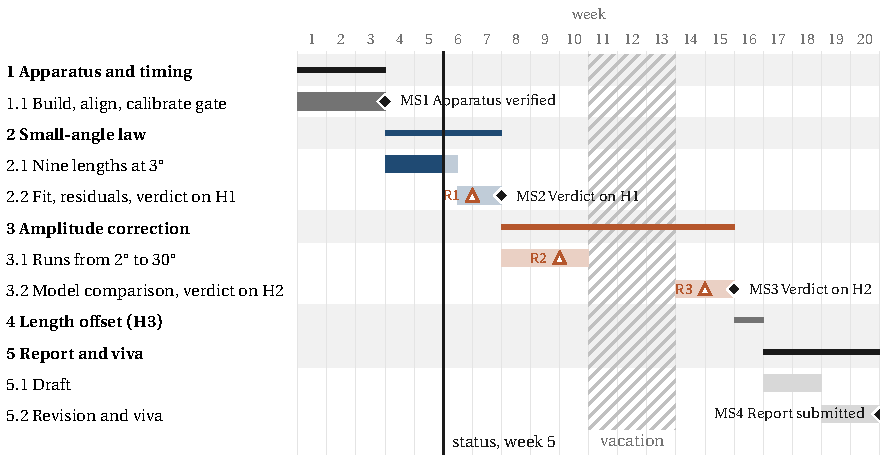
\includegraphics[width=\linewidth]{figures/gantt}
  \caption{\lead{Gantt chart of the project.} Bars are dark where the work is done by the status line and pale where it is planned; hatched weeks are vacation. Diamonds are milestones and triangles are the risk triggers of \cref{tab:risks}.}
  \label{fig:gantt}
\end{figure}

% The milestones of the Gantt chart, each with its week.
\begin{milestones}
  \item MS1, apparatus verified: week 3, done.
  \item MS2, verdict on \badge{H1}: week 7.
  \item MS3, verdict on \badge{H2}: week 15.
  \item MS4, report submitted: week 20.
\end{milestones}

% A wide table of words: bands on alternate rows, levels as chips, and each
% hypothesis a risk threatens as its badge.
\section{Risks}

\Cref{tab:risks} gives each risk a trigger, the check that shows whether it has come true, and the week that check falls in.

\begin{table}[tbp]
  \caption{\lead{Risks and fallbacks.} Each trigger is the check that shows whether the risk has come true, with its week, marked R1 to R3 in \cref{fig:gantt}.}
  \label{tab:risks}
  \begin{tabularx}{\linewidth}{l >{\raggedright\arraybackslash}X l l l >{\raggedright\arraybackslash}X >{\raggedright\arraybackslash}X}
    \toprule
    \multicolumn{2}{l}{\head{Risk}} & \head{Threatens} & \head{Likely} & \head{Impact} & \head{Trigger} & \head{Fallback} \\
    \midrule
    \textbf{R1} & timing drifts between runs & \badge{H1} & \level{low} & \level{high} & $\chi^2/\nu > 2$, week 6 & repeat two lengths \\
    \band \textbf{R2} & amplitude read too coarsely & \badge{H2} & \level{medium} & \level{medium} & spread over \qty{0.5}{\degree}, week 9 & film the release \\
    \textbf{R3} & correction too simple & \badge{H2} & \level{medium} & \level{high} & residuals trend above \qty{20}{\degree}, week 14 & fit below \qty{15}{\degree} only \\
    \band \textbf{R4} & illness, lost weeks & schedule & \level{medium} & \level{medium} & a task a week late, any week & drop \badge{H3} \\
    \bottomrule
  \end{tabularx}
\end{table}

Each trigger is checked in its week at the meeting with the supervisor. When one fires, the plan moves to its fallback for the weeks that remain and the Gantt chart is redrawn with the new dates. The fallback for R4 drops \badge{H3}, the hypothesis the aim depends on least.

\bibliographystyle{apsrev4-2}
\bibliography{refs}

\end{document}
